\chapter{Tinjauan Pustaka dan Dasar Teori}

\section{Tinjauan Pustaka}

\subsection{Apakah Pola Deteksi Duplikat (CDP) dapat Disalin}
CDP dinilai dapat digunakan untuk mendeteksi pemalsuan, sehingga akhir-akhir ini mendapatkan banyak perhatian dari akademisi dan industri. Tingkat keamanan CDP dalam mendeteksi serangan pemalsuan yang canggih telah dipelajari secara teoritis dan praktis dalam beberapa penelitian, namun hasilnya masih belum sepenuhnya meyakinkan \cite{PICARDCANCOPYDETECTIONPATTERN}. Kontribusi utama dari penelitian ini adalah untuk menyajikan kumpulan data CDP secara publik dan berbagai jenis contoh penyerangan terdapat CDP tersebut, sehingga kinerja CDP terhadap beberapa penyerangan dapat diketahui. Set data CDP tersebut terdiri dari lebih dari 27.500 gambar CDP dan merupakan set data CDP terbesar hingga saat ini \cite{PICARDCANCOPYDETECTIONPATTERN}. Kontribusi selanjutnya adalah meneliti tentang kinerja detektor CDP dalam mendeteksi CDP asli ataupun salinan. Verifikasi dari CDP dapat dilakukan dengan perangkat seluler, tanpa harus menggunakan pemindai khusus \cite{WONG2017}, \cite{SCHRAML2018REAL}. Dengan dataset dan detektor yang dibuat, peneliti sebelumnya ingin menguji validitas hipotesis bahwa CDP yang dicetak berulang kali akan terdegradasi kualitasnya dan dapat dideteksi sebagai CDP palsu \cite{PICARDCANCOPYDETECTIONPATTERN}. Kontibusi terakhir dari penelitian ini adalah beberapa metode yang dapat dilakukan untuk meningkatkan performa klasifikasi dari model. 

\begin{figure}[h]
	\centering
	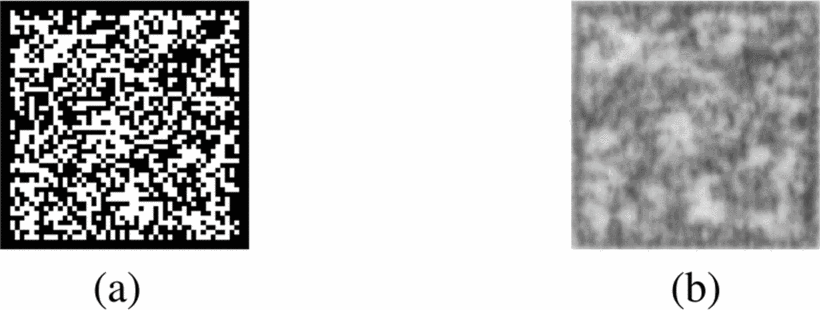
\includegraphics[width=10cm]{contents/chapter-2/2-cdporivsfake.png}
	\caption{Contoh dari CDP a) CDP original hasil \emph{generate} dari program $I$ b) CDP yang telah terdegradasi kualitasnya akibat dari beberapa kali penyetakan dan pemindaian $\widetilde{I}$ \cite{PICARDCANCOPYDETECTIONPATTERN}}
	\label{Fig: 2-cdporivsfake}
\end{figure}

\subsubsection{Prinsip Degradasi Informasi}
Prinsip dari deteksi CDP palsu dilakukan berdasarkan hilangnya informasi, yang mana muncul dari proses pemindaian dan penyetakan \cite{picard2004digital}. Proses \emph{Print-and-Scan} (P\&S) merupakan proses stokastik (mempunyai unsur peluang atau kebolehjadian) \cite{phan2014document}, yang menyebabkan perubahan struktur dan kualitas gambar pada CDP, seperti yang ditampilkan pada Gambar \ref{Fig: 2-cdporivsfake} \emph{Noise} yang dihasilkan dari P\&S CDP sulit untuk dikarakterisasi \cite{picard2008security} karena setiap printer dan pemindai memiliki karakteristiknya sendiri.

\begin{figure}[h]
	\centering
	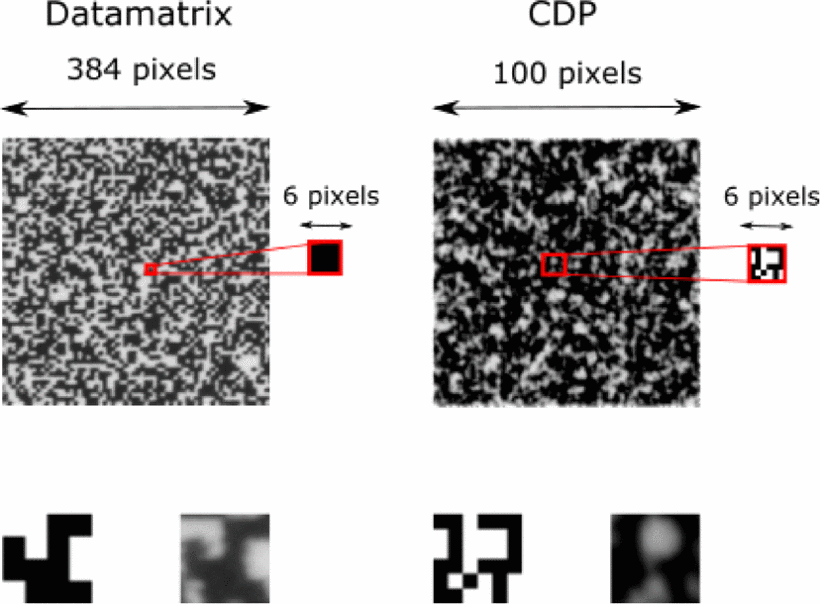
\includegraphics[width=10cm]{contents/chapter-2/2-datamatrixvscdp.png}
	\caption{Perbandingan dari CDP dengan data-matriks: Data-matriks memiliki ukuran unit komponen yang lebih besar, sehingga degradasi informasi tidak berdampak signifikan pada struktur kode \cite{PICARDCANCOPYDETECTIONPATTERN}}
	\label{Fig: 2-datamatrixvscdp}
\end{figure}

CDP sering dibandingkan dengan kode batang dua dimensi seperti data-matriks karena kemiripan visualnya. Namun, seperti yang diilustrasikan pada Gambar \ref{Fig: 2-datamatrixvscdp}, unit elemen data-matriks jauh lebih besar dibandingkan unit elemen CDP. Oleh karena itu, prinsip kehilangan atau degradasi informasi tidak berdampak pada struktur data-matriks. Sebagai contoh, korelasi antara data-matriks digital \emph{template} hasil \emph{generate} dengan versi rusak P\&S bisa lebih dari $0,9$, sedangkan korelasi antara CDP digital \emph{template} hasil \emph{generate} dengan versi rusak P\&S-nya hanya sekitar $0,45-0,55$ tergantung pada pemindai dan penyetaknya. Oleh karena itu, ukuran dari unit elemen pola CDP, yaitu $uxu$ piksel seperti yang ditampilkan pada Gambar \ref{Fig: 2-datamatrixvscdp}, ukuran pola keseluruhan juga sangat mempengaruhi proses otentikasi dan kemampuan pemalsu dalam mereproduksi pola. Pada praktiknya, ukuran unit elemen pada CDP adalah $1x1$ piksel atau $2x2$ piksel agar bisa memanfaatkan prinsip kehilangan atau degradasi informasi secara maksimal.

\subsubsection{Definisi Teoritis dari Sistem Autentikasi CDP}
Autentikasi dari CDP terdiri dari dua langkah utama. Langkah pertama adalah langkah registrasi di mana pola dihasilkan kemudian dicetak dengan penyetak untuk menghasilkan CDP asli. Langkah kedua adalah verifikasi CDP, menggunakan sebuah perangkat pemindai yang telah terotentikasi (perangkat selular dengan kamera), CDP dipindai dan dilewatkan ke tes autentikasi (dengan parameter-parameter peminadaian tertentu). Jika tes tersebut positif, item dianggap autentik.

Upaya penyerangan yang paling sering terjadi oleh pembajak adalah sebagai berikut: Pembajak melakukan pemindaian CDP pada sebuah item menggunakan pemindai beresolusi tinggi, mengestimasi pola asli dari CDP, kemudian mencetak pola yang telah diestimasi menggunakan penyetak beresolusi tinggi. Pada skenario ini $I$ merupakan CDP digital hasil \emph{generate} dari \emph{template}, kemudian $\Pi(I)$ merupakan hasil \emph{generate} CDP \emph{template} yang dicetak, dengan $\Pi(\cdot)$ \emph{noise} yang dihasilkan dalam proses penyetakan menggunakan penyetak yang telah terautentikasi. Selanjutnya, proses autentikasi dapat dirumuskan sebagai uji hipotesis berikut ini:

\begin{align}
	&\mathcal{H}_{0}:\tilde{I}\sim\Sigma(\Pi(I)),\\ &\mathcal{H}_{1}:\tilde{I}\not\sim\Sigma(\Pi(I)),\nonumber
\end{align}

\noindent di mana $\widetilde{I}$ adalah gambar CDP \emph{grayscale} yang diterima oleh pusat autentikasi. $\widetilde{I}$ dapat berupa CDP asli (i.e. $\Sigma(\Pi(I))$) atau CDP palsu (i.e. $\Sigma(\Pi'(\hat{I}))$). Metriks yang digunakan untuk membandingkan CDP asli dengan palsu adalah koefisien jarak ataupun korelasi \cite{dirik2012copy}.

\subsubsection{Komponen dari Detektor}
Hasil menunjukkan bahwa autentikasi menggunakan CDP \emph{raw grayscale} lebih efisien dibandingkan dengan CDP yang telah di-\emph{thresholding} \cite{phan2014document}. Kemudian, secara umum, ada beberapa langkah yang dilakukan untuk melakukan autentikasi CDP, antara lain:

\begin{itemize}
	\item Melakukan \emph{resizing} pada \emph{template} CDP menggunakan faktor skala tertentu.
	\item Menggunakan teknik pencocokan \emph{template} dengan mengambil sub-bagian dari CDP.
	\item Menggunakan \emph{high pass filtering} (seperti \emph{unsharp masking}) sebelum melakukan penyekoran korelasi.
\end{itemize}

\subsection{Detekti Pembajakan menggunakan SQR}
Pendekatan keamanan tradisional pada produk sebelumnya sudah diimplementasikan melalui \emph{taggant}, hologram, dan tinta keamanan.Beberapa metode tersebut memang mudah diimplementasikan, mudah diverifikasi, dan murah. Namun, dalam sebuah Kode QR metode-metode tersebut belum dapat diimplementasikan. Produk yang ditempeli oleh kode QR palsu biasanya masih dapat dipindai dan mengembalikan keluaran sama dengan produk asli. Penelitian yang dilakukan oleh Justin Picard, Paul Landry, dan Michael Bolay ini membahas tentang bagaimana mengimplementasikan CDP ke dalam SQR untuk mendeteksi pembajakan \cite{picard2021counterfeit}.

\begin{figure}[h]
	\centering
	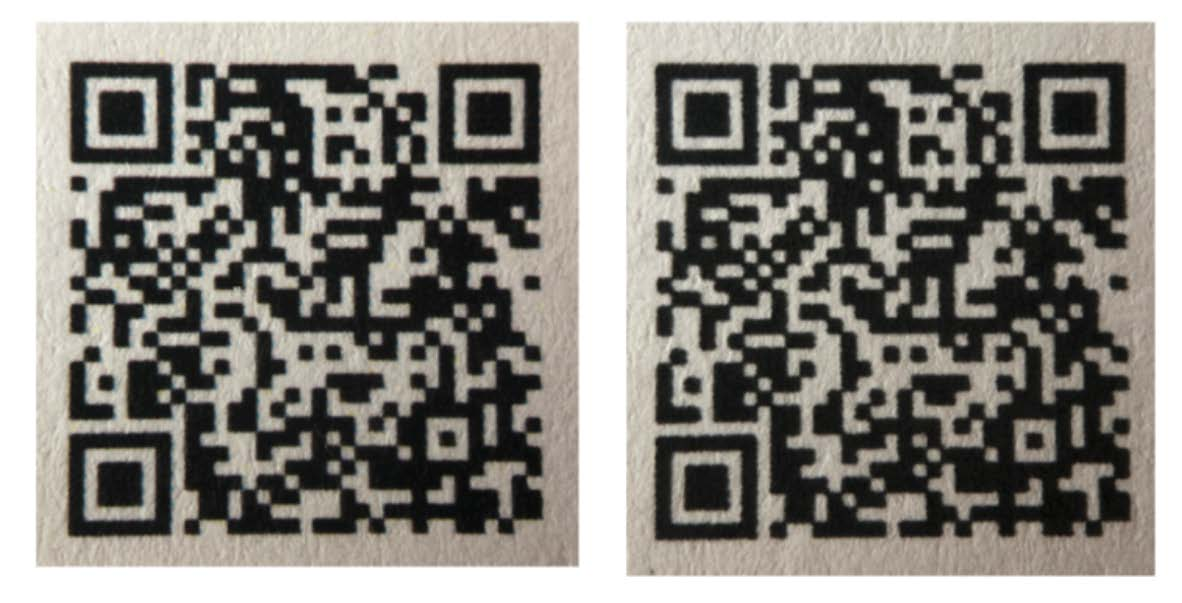
\includegraphics[width=10cm]{contents/chapter-2/2-qrorivspalsu.jpg}
	\caption{Perbandingan dari kode QR asli dan palsu, keduanya menyimpan informasi yang sama dan sama-sama dapat dipindai \cite{picard2021counterfeit}}
	\label{Fig: 2-qrorivspalsu}
\end{figure}

Pada Gambar \ref{Fig: 2-qrorivspalsu} terlihat bahwa sangat sulit untuk membedakan antara kode QR asli dan replika, apabila jika tidak ada pembandingnya. Skenario yang dapat dilakukan oleh pembajak dalam menerbitkan kode QR palsu dapat dilihat pada Gambar \ref{Fig: 2-counterveiterpractice}. Kode QR palsu dipindai dengan perangkat beresolusi tinggi, kemudian dicetak ulang. Harapannya dengan CDP yang diletakkan pada kode QR, kode QR palsu yang dipindai untuk autentikasi dapat terdeteksi sebagai kode QR palsu, lihat pada Gambar \ref{Fig: 2-counterveiterpractice}.

\begin{figure}[h]
	\centering
	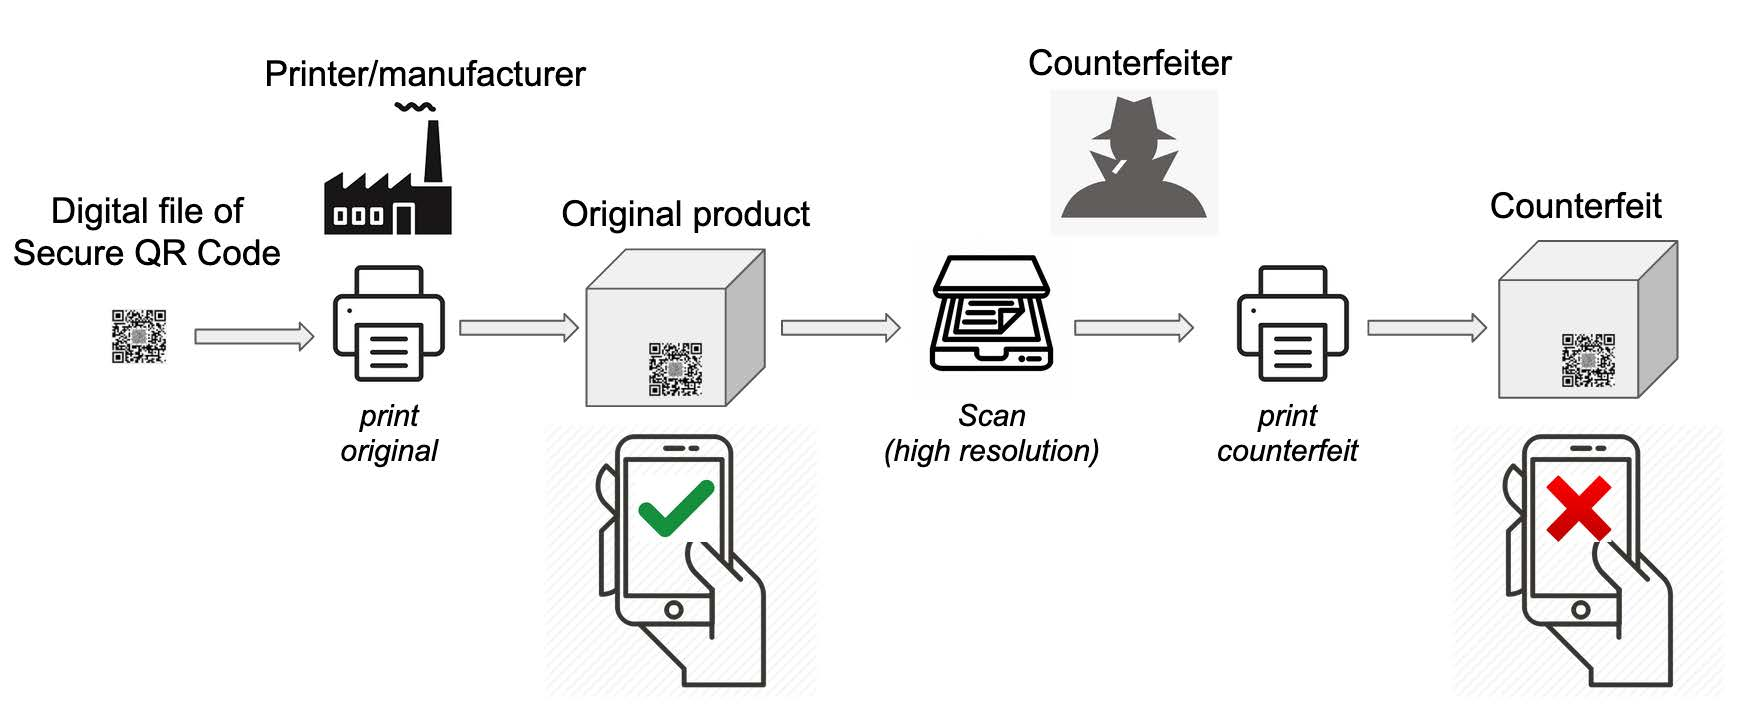
\includegraphics[width=10cm]{contents/chapter-2/2-counterveiterpractice.jpg}
	\caption{SQR diharapkan dapat mendeteksi kode QR palsu pada saat diautentikasi oleh pengguna \cite{picard2021counterfeit}}
	\label{Fig: 2-counterveiterpractice}
\end{figure}

\subsubsection{Struktur dari SQR}
\begin{figure}[h]
	\centering
	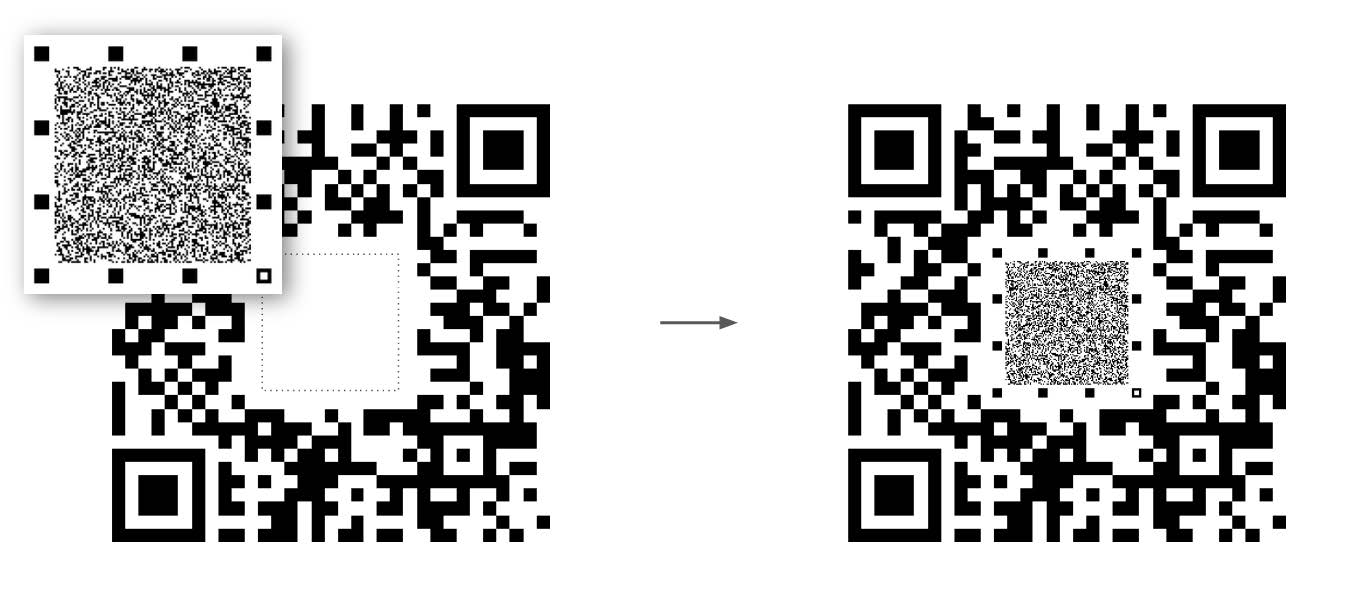
\includegraphics[width=10cm]{contents/chapter-2/2-struktursqr.jpg}
	\caption{Struktur SQR secara umum \cite{picard2021counterfeit}}
	\label{Fig: 2-struktursqr}
\end{figure}

Secara umum, CDP akan diletakkan di tengah-tengah dari kode QR. CDP nantinya akan digunakan untuk proses autentikasi. Di sekitar CDP diletakkan beberapa \emph{markers} untuk memudahkan program dalam mendeteksi dan mendapatkan objek CDP. CDP mungkin ditempelkan di tengah-tengah kode QR karena adanya fitur koreksi kesalahan dalam kode QR. Ada empat jenis koreksi kesalahan pada kode QR: L, M, Q, dan H, yang secara teoritis memiliki kemampuan untuk memulihkan informasi yang hilang sebesar 7\%, 15\%, 25\%, dan 30\% kerusakan pada kode QR. Pada penelitian ini, area yang dirusak untuk meletakkan CDP adalah sebesar 1/9 dari ukuran awal kode QR. Aplikasi yang digunakan untuk melakukan autentikasi pada perangkat pemindai (perangkat seluluer) hanya mengambil objek CDP saja, hal tersebut memiliki beberapa keuntungan, area yang digunakan untuk autentikasi menjadi lebih spesifik, sehingga kecepatan deteksi akan lebih cepat, fokus dari kamera juga relatif akan lebih baik karena mengambil objek yang lebih kecil dan terfokus, selain itu karena sistem autentikasi berada di \emph{remote server} yang mana data akan dikirim dari perangkat seluler pemindai, maka semakin kecil area yang dikirimkan, semakin hemat \emph{bandwith} yang digunakan.

\subsubsection{Pembuatan dan Pencetakan SQR}
CDP yang digunakan dalam penelitian ini menggunakan dua kuantisasi \emph{grayscale} atau biner. Resolusi mesin \emph{printer} yang digunakan adalah 812,8 ppi dengan merek HP Indigo. CDP di-\emph{generate} menggunakan \emph{pseudo-random number generator}, menggunakan \emph{seed} tertentu. CDP dapat dibuat unik untuk setiap kode QR ataupun sama pada sekelompok kode QR tertentu. Dalam melakukan penyetakan dan pemindaian SQR, perangkat pencetak dan pemindai akan diverifikasi terlebih dahulu dengan konfigurasi dan parameter tertentu untuk menjamin kualitas dari pencetakan.

\subsubsection{Autentikasi SQR}
Perangkat pemindai QR biasa sudah pasti dapat melakukan \emph{decode} informasi dari kode QR, namun untuk melakukan autentikasi terhadap CDP, tentunya diperlukan aplikasi khusus. Aplikasi khusus ini berjalan di perangkat seluler, secara umum proses pemindaian yang dilakukan oleh aplikasi khusus tersebut adalah sebagai berikut:

\begin{itemize}
	\item Aplikasi akan melakukan pemindaian per-\emph{frame} dari kamera hingga mendapatkan kode QR.
	\item Kode QR akan di-\emph{decode} untuk mengekstrak informasi dalam kode QR.
	\item Indeks kualitas pemindaian akan dikalkulasi berdasarkan \emph{frame} yang didapatkan.
	\item Jika indeks kualitas pemindaian dinilai cukup tinggi, area CDP akan dideteksi, dipotong, dan dikirim ke \emph{remote server} bersamaan dari informasi dari kode QR yang telah ter-\emph{decode} untuk autentikasi.
\end{itemize}

\begin{figure}[h]
	\centering
	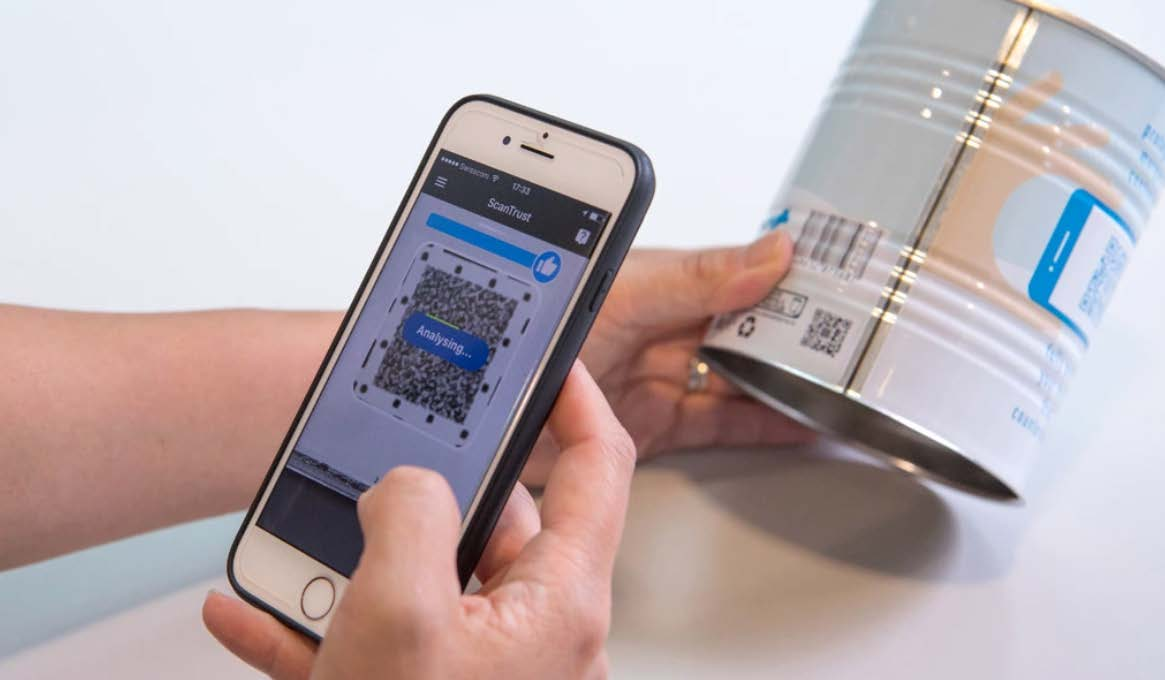
\includegraphics[width=10cm]{contents/chapter-2/2-pemindaiansqr.jpg}
	\caption{Perangkat seluler melakukan pemindaian menggunakan aplikasi khusus \cite{picard2021counterfeit}}
	\label{Fig: 2-pemindaisqr}
\end{figure}

Setelah \emph{server} mendapatkan CDP yang telah dipotong beserta informasi data kode QR, autentikasi yang dilakukan di \emph{server} adalah sebagai berikut:

\begin{itemize}
	\item \emph{Identifier} unik akan diekstrak dari informasi kode QR yang didapatkan yang mana dibutuhkan sebagai parameter autentikasi.
	\item Template CDP digital akan di-\emph{generate}.
	\item Matriks similaritas akan dikalkulasi dari perbandingan antara CDP yang dikirimkan dari hasil pemindaian dengan CDP \emph{template} yang di-\emph{generate}.
	\item Penyesuaian lain seperti, ketajaman gambar, filter akan dilakukan untuk memperoleh hasil terbaik.
	\item Normalisasi nilai akan dilakukan.
	\item Keluaran berupa CDP "asli", "palsu", atau "pemindaian buruk" akan dikeluarkan oleh \emph{server} (pemindaian buruk bisa disebabkan oleh hasil gambar yang blur).
\end{itemize}

\subsection{Autentikasi Digital menggunakan CDP}

\subsection{Pencetakan Variasi CDP}

\subsection{Autentikasi CDP menggunakan Perangkat Seluler}

\section{Dasar Teori}

\subsection{Kode QR}

Kode QR (Quick Response) adalah sebuah kode matriks dua dimensi (2-D) yang dapat dibaca oleh komputer. Kode QR dua dimensi dapat menyimpan data yang lebih banyak dibandingkan dengan kode satu dimensi (barcodes) dengan ruang yang lebih kecil. Selain itu, kode QR memiliki fitur koreksi kesalahan pembacaan dan beberapa fitur unik lainnya \cite{densoqrcode}. 

Seperti bahasa tertulis lainnya, kode batang atau \emph{barcode} merupakan representasi visual dari informasi. Namun, berbeda dengan bahasa yang dapat dibaca oleh manusia, kode batang dirancang untuk dibaca dan dipahami oleh komputer atau mesin. Menggunakan sistem penglihatan dari mesin berupa pemindai laser optik ataupun kamera dan perangkat lunak yang dapat menginterpretasikan kode batang. Aturan bagaimana \emph{barcode} dikonstruksikan disebut sebagai \emph{grammar}, sedangkan set karakter yang digunakan (alfabet) disebut \emph{symbology} \cite{densoqrcode}.

\subsubsection{Bagaiamana Kode QR Bekerja}
\begin{figure}[h]
	\centering
	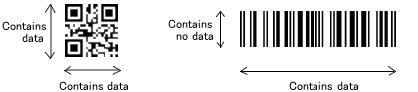
\includegraphics[width=10cm]{contents/chapter-2/2-2dvs1dcode.jpg}
	\caption{Perbandingan 1-D dengan 2-D \emph{barcodes}}
	\label{Fig: 2-2dvs1dcode}
\end{figure}

Tidak seperti kode batang satu dimensi, kode QR adalah matriks 2-D yang menyimpan informasi dalam tiap modul di baris dan kolomnya yang memiliki gelap dan terang tertentu.

\begin{figure}[h]
	\centering
	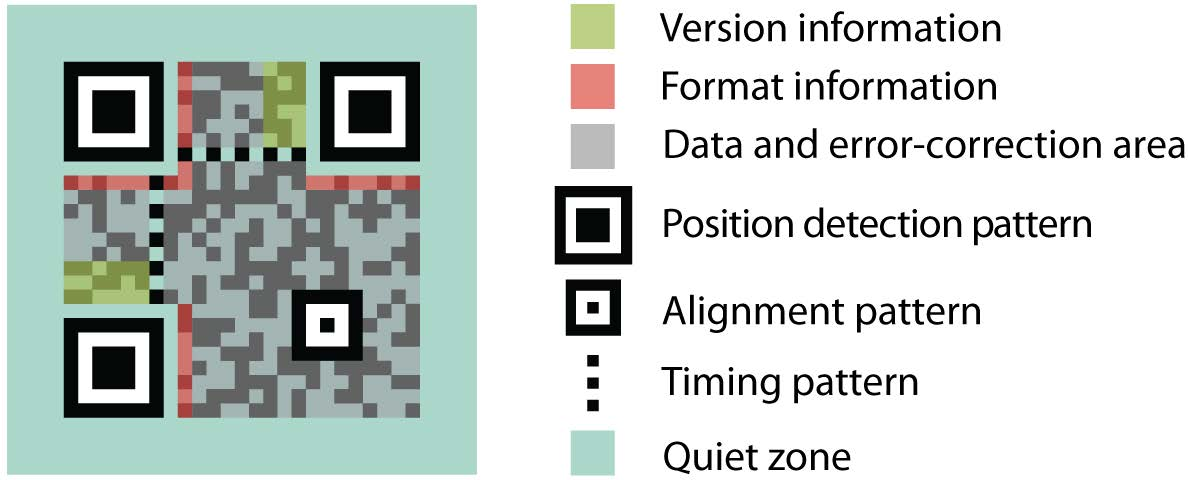
\includegraphics[width=10cm]{contents/chapter-2/2-strukturqrasli.jpg}
	\caption{Struktur modul pada kode QR dua dimensi}
	\label{Fig: 2-strukturqrasli}
\end{figure}

Setiap modul dalam kode QR memiliki fungsi-fungsi tertentu. Beberapa modul berisi tentang informasi yang tersimpan dalam kode QR itu sendiri, dengan lainnya dibagi menjadi beberapa grup berdasarkan fungsinya. Untuk memastikan kode QR dapat dipindai dari berbagai sisi, ada tiga modul \emph{position detection pattern} yang terletak di ketiga sudut yang memungkinkan kode QR untuk dipindai dari 360$^{\circ}$.

\subsubsection{Versi Kode QR}
Kode QR dapat di-\emph{generate} dari 40 versi yang berbeda, dari yang berukuran $21x21$ modul (versi 1) hingga $177x177$ modul (versi 40).

\begin{figure}[h]
	\centering
	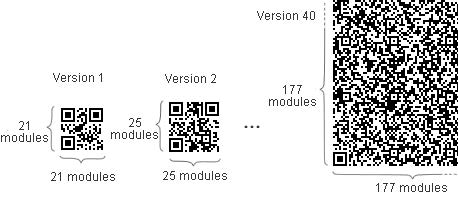
\includegraphics[width=10cm]{contents/chapter-2/2-versiqr.jpg}
	\caption{Jumlah modul berdasarkan versi kode QR}
	\label{Fig: 2-versiqr}
\end{figure}

Setiap kenaikan satu versi, maka akan ada penambahan 4 modul, sehingga dapat memuat data atau informasi yang lebih banyak. Jumlah maksimum data yang dapat disimpan tergantung pada versi kode QR, tipe karakter, dan besar toleransi kesalahan.

\subsubsection{Koreksi Kesalahan Kode QR}
Koreksi kesalahan kode QR mengimplementasikan \emph{Reed-Solomon codes}, yang mana merupakan salah satu metode koreksi kesalahan matematis yang banyak digunakan. Hal ini memungkinkan kode QR tetap dapat dibaca walaupun dalam kondisi kotor ataupun rusak dengan batasan tertentu. Ada empat tipe koreksi kesalahan standar yang ada dalam kode QR. Semakin tinggi level koreksi kesalahan, semakin besar toleransi terhadap kerusakan kode QR, namun semakin besar juga versi kode QR-nya.

\begin{table}[h]
	\caption{Tabel perbandingan level koreksi kesalahan dengan persentase toleransi kesalahannya}
	\vspace{0.5em}
	\centering
	\begin{tabular}{|c|c|c|}
		\hline
		Level Koreksi Kesalahan & Besar Toleransi Kesalahan \\
		\hline
		L & 7\% \\
		M & 15\% \\
		Q & 25\% \\
		H & 30\% \\ \hline
	\end{tabular}
	\label{Tab: 2-tabelperbandinganlevelkoreksi}
\end{table}

Dalam memilih level koreksi kesalahan, sebaiknya disesuaikan dengan kondisi lingkungan di mana kode QR tersebut digunakan. Misalnya dalam kondisi lingkungan yang bersih, level L (7\%) dapat digunakan. Secara umum, level yang paling sering digunakan adalah level M (15\%).

\subsection{Deteksi Pola Duplikat (CDP)}
Pola deteksi duplikat (CDP) adalah sebuah gambar berpola dengan entropi tinggi yang dibuat menggunakan kode rahasia (\emph{secret key}). CDP memanfaatkan konsep dari "\emph{information loss principle}" dari proses P\&S pada dokumen. Biasanya, CDP digunakan di dalam gambar digital yang dicetak ataupun langsung ke dalam dokumen digitalnya. CDP tidak didesain untuk dideteksi menggunakan mata telanjang. Namun, CDP dapat bekerja secara maksimal pada pendeteksian otomatis pada gambar yang dipindai. CDP akan sangat bermanfaat saat digunakan dalam memverifikasi dokumen dalam jumlah besar \cite{picard2004digital}, \cite{picard2004towards}, \cite{}.

\begin{figure}[h]
	\centering
	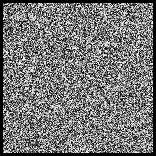
\includegraphics[width=3cm]{contents/chapter-2/2-contohcdp.jpg}
	\caption{Salah satu contoh CDP}
	\label{Fig: 2-contohcdp}
\end{figure}

CDP telah dicoba untuk dicetak menggunakan berbagai variasi \emph{printers}: \emph{Printer} kantor seperti \emph{inkjet} dan \emph{laser}, \emph{printer offset} dan \emph{digital offset}, dan juga \emph{printer} termal. Hasil percobaan dari pencetakan menggunakan beberapa jenis \emph{printer} tadi, semua CDP salinan dapat dibedakan dengan CDP asli dengan margin yang cukup nyaman \cite{picard2004digital}, \cite{picard2004towards}.

CDP sebaiknya tidak dianggap sebagai pesaing untuk perangkat keamanan optik lainnya, namun dijadikan sebagai alternatif yang lebih murah pada kasus-kasus tertentu. Dengan memanfaatkan konsep degradasi gambar dan informasi yang tidak terancam oleh perkembangan perangkat pemindai dan pencetak digital, CDP menjadi alternatif yang paling murah dalam memroteksi dokumen \cite{picard2004digital}, \cite{picard2004towards}, \cite{harwood1998optical}.

\subsection{Lokalisasi Objek dengan Pengenalan Pola}
Lokalisasi objek adalah proses mengidentifikasi posisi dan orientasi objek atau pola tertentu pada sebuah gambar menggunakan teknik pengolahan citra dan visi komputer. Proses ini melibatkan deteksi objek atau pola dalam gambar serta mengestimasi lokasi dan orientasi yang tepat relatif terhadap kamera \cite{sivic2003video}, \cite{liu2016ssd}.

Berbagai teknik telah diusulkan untuk melakukan lokalisasi objek atau gambar dengan pengenalan pola, termasuk deteksi fitur, pencocokan \emph{template}, dan metode berbasis pembelajaran mesin. Teknik-teknik ini telah digunakan dalam berbagai aplikasi, seperti \emph{augmented reality}, robotika, dan pelacakan objek.

\subsection{ArUco \emph{Marker}}
ArUco \emph{marker} adalah jenis \emph{marker} fidusial yang biasa digunakan untuk estimasi pose kamera dan pelacakan dalam pengolahan citra dan visi komputer. ArUco \emph{marker} terdiri dari kisi-kisi kotak hitam dan putih dengan pola unik yang mudah dideteksi dan dikenali oleh algoritma visi komputer. ArUco \emph{marker} banyak digunakan dalam aplikasi robotika, realitas tambahan, dan pelacakan objek karena kesimpelannya, akurasi deteksi yang tinggi, dan biaya komputasi yang rendah.

\emph{Marker} fidusial adalah objek berpola yang digunakan ke dalam sebuah gambar atau tempat tertentu untuk memudahkan sistem visi komputer menentukan posisi dan orientasi objek atau \emph{scene} dengan akurasi yang tinggi. \emph{Marker} fidusial biasanya didesain dengan pola atau bentuk yang unik dan mudah dikenali, sehingga dapat dideteksi dan dilacak oleh algoritme pendeteksian objek visi komputer, yang memungkinkan estimase pose dan pelacakan yang akurat. \emph{Marker} fidusial banyak digunakan dalam berbagai aplikasi seperti \emph{augmented reality}, robotika, dan pendeteksian objek.

% \subsection{Ekstraksi Fitur pada Gambar}

\subsection{Koefisien Jarak}
Koefisien jarak merupakan ukuran atau besaran yang menggambarkan seberapa dekat atau jauh dua objek dalam ruang atau dimensi tertentu. Koefisien jarak dapat digunakan untuk mengukur kesamaan atau perbedaan antara dua objek yang diamati. Ada beberapa koefisien jarak yang sering digunakan, antara lain:

\subsubsection{Koefisien Jarak Euclidean}
Jarak Euclidean adalah ukuran jarak yang paling umum digunakan dalam matematika dan ilmu komputer untuk mengukur jarak antara dua titik dalam ruang Euclidean n-dimensi. Jarak Euclidean dihitung sebagai akar kuadrat dari jumlah kuadrat perbedaan koordinat antara dua titik.
Secara formal, jarak Euclidean antara dua vektor $\mathbf{u}$ dan $\mathbf{v}$ dalam ruang Euclidean n-dimensi didefinisikan sebagai:

\begin{equation}
  d(\mathbf{u},\mathbf{v}) = \sqrt{\sum_{i=1}^{n}(u_i - v_i)^2}
\end{equation}

\noindent di mana $n$ adalah jumlah dimensi dalam \emph{vector space}, dan $u_i$ dan $v_i$ merepresentasikan komponen ke-$i$ pada vektor.

\subsubsection{Koefisien Jarak Korelasi}
Koefisien jarak korelasi adalah suatu ukuran kemiripan atau perbedaan antara dua vektor, berdasarkan korelasi antara komponen-komponennya. Nilai dari jarak korelasi dinormalisasi antara 0 dan 1, di mana 0 menunjukkan korelasi positif sempurna sedangkan 1 menunjukkan korelasi negatif sempurna.

Untuk menghitung jarak korelasi antara dua vektor $u$ dan $v$, dapat dituliskan dengan:

\begin{equation}
	d = 1-\frac{(u-\bar{u})\cdot (v-\bar{v})}{\Vert(u-\bar{u})\Vert_2\Vert(v-\bar{v})\Vert_2}
\end{equation}

\noindent di mana $d$ adalah jarak korelasi antara $u$ dan $v$, $\bar{v}$ adalah rata-rata elemen dari vektor $v$, dan $x\cdot y$ adalah \emph{dot product} dari $x$ dan $y$. Jarak korelasi sering digunakan dalam algoritma pengelompokan dan klasifikasi untuk mengukur perbedaan antara sampel, terutama ketika vektor memiliki banyak komponen dan data sangat berkorelasi.

\subsubsection{Koefisien Jarak Kosinus}
Koefisien jarak kosinus adalah sebuah metode untuk mengukur kemiripan antara dua vektor dalam ruang n-dimensi \cite{schutze2008introduction}, \cite{deisenroth2020mathematics}. Metode ini mengukur sudut antara dua vektor dan menghasilkan nilai berkisar antara 0 dan 1, di mana 0 menunjukkan bahwa vektor tersebut saling tegak lurus, sedangkan 1 menunjukkan bahwa vektoor tersebut saling sejajar. Semakin kecil nilai koefisien jarak kosinus, semakin mirip kedua vektor tersebut. Jarak kosinus antara dua vektor $u$ dan $v$ dapat dituliskan sebagai berikut:

\begin{equation}
	1-\frac{u\cdot v}{\Vert u\Vert_2\Vert v\Vert_2}
\end{equation}

\noindent di mana $u\cdot v$ adalah hasil \emph{dot product} antara vektor $u$ dan $v$, sedangkan $\Vert u\Vert_2$ dan $\Vert v\Vert_2$ adalah panjang dari vektor $u$ dan $v$.

\subsubsection{Koefisien Jarak Canberra}
Jarak Canberra adalah salah satu metode mengukur jarak antara dua vektor dalam ruang n-dimensi. Metode ini mengevaluasi perbedaan proporsional antara nilai-nilai pada setiap elemen vektor. Metode ini sering digunakan dalam analisis data untuk mengukur kemiripan antara dua set data numerik \cite{clusteringSumayiaAlAnazi}, \cite{sneath1973numerical}. Secara formal, perhitungan jarak canberra antara dua vektor $u$ dan $v$ adalah:

\begin{equation}
	d(u,v)=\sum_i\frac{\left | u_i-v_i \right |}{\left | u_i \right |+\left | v_i \right |}
\end{equation}

\subsection{Transformasi Homografi}
Transformasi homografi adalah sebuah transformasi geometri pada ruang n-dimensi yang memetakan setiap titik pada bidang ke titik yang sesuai pada bidang lainnya, dengan menerapkan konsep persamaan linier homogen. Transformasi homografi dapat mengubah ukuran, rotasi, dan persepektif dari gambar atau objek pada bidang ruang n-dimensi.

Transformasi homografi biasanya dilakukan dalam ruang koordinat \emph{homogeneous}, yang merupakan ruang n+1 dimensi dengan koordinat homogen yang memungkinkan dilakukannya transformasi perspektif. Dalam ruang koordinat \emph{homogeneous}, sebuah titik pada bidang n-dimensi dinyatakan dalam bentuk vektor homogen (x, y, z, w), di mana x, y, dan z adalah koordinat euclidean, dan w adalah koordinat homogen. Sebuah matriks homografi H juga dinyatakan dalam bentuk matriks homogen:

\begin{equation}
	\begin{bmatrix}
		x'\\ 
		y'\\ 
		w'
		\end{bmatrix}=H\begin{bmatrix} 
		x\\ 
		y\\ 
		w
		\end{bmatrix}
\end{equation}

\subsection{Pembelajaran Mesin}


\section{Analisis Perbandingan Metode}